\documentclass[../main.tex]{subfiles}
\usepackage{graphicx}
\usepackage{subcaption}
\usepackage{adjustbox}

\begin{document}

\begin{enumerate}
    \item 
    \item 
\end{enumerate}

\subsection*{Imágenes del equipo utilizado}

\begin{figure}[H]

    \begin{tabular}{c c}
        
    \begin{subfigure}{0.5\textwidth} 
        \centering
        %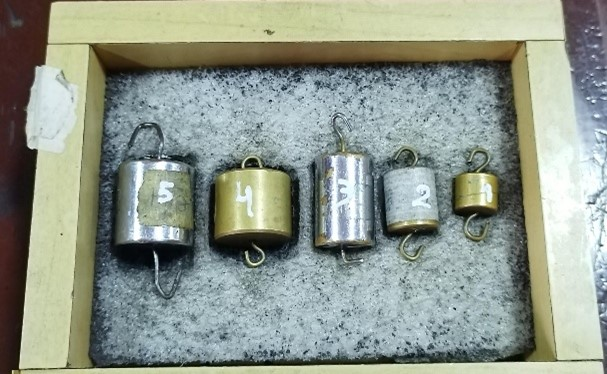
\includegraphics[width=0.8\linewidth, height=3.5cm]{images/materiales/mat1.jpg}
        \caption{Pesas}
        \label{fig:pesas}
    \end{subfigure}
   
    \end{tabular}
    
    \caption{Materiales utilizados.}
    \label{fig:materiales}
\end{figure}

\end{document}